\subsection{State of the art SLAM}
\label{chap:slam}
As mentioned before, SLAM describes the field of problem where an agent or robot has to locate itself
in an unknown environment. Therefore the agent has to build up a map. The map normally containing discrete 
landmarks but also continuous functions or planes (as an approximation of the world) could be possible. 
All of the techniques have in common, that the created map is always an estimation. So SLAM is a 
probabilistic approach. The reason for that is, that all data given is uncertain. Such as current 
position, measured value (e.g. magnetic field) or landmark position. The noise of the measurements is 
normally gaussian distributed. 

When thinking of SLAM there are two common classifications \cite{grisetti_tutorial_2010}. The first 
class models SLAM as an on-line state estimator, where the state is the current position of the robot 
within the map. This approach is called filtering or on-line SLAM. In contrast to that smoothing 
approaches attempt to estimate the full trajectory of the robot based on all measurements. 
Often smoothing is called full SLAM.

Regardless of filtering or smoothing approaches, they often using Kalman or particle filter to estimate
the current state \cite{grisetti_tutorial_2010}. Kalman filter is a mathematical concept and is also known
as linear quadratic estimation (LQE). It contains two major steps, prediction and update.
In the prediction step the next state is predicted by using the currently given data. After that, 
the prediction will be improved by combining the estimated state from the prediction with the new 
measured state \cite{kalman_filter_2001}. This step is called update. Kalman filter always follow only one
hypothesis. In contrast to that particle filters where invented. Each particle follows a specific
hypothesis and normally there are multiple particles. So, particle filter follow multiple hypothesis.

\begin{figure}[h!]
	\centering
	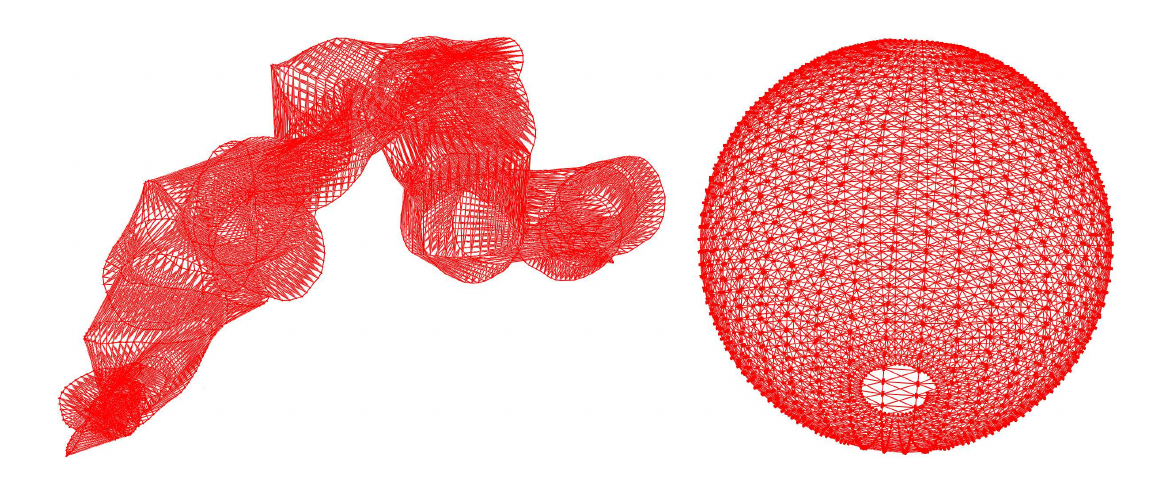
\includegraphics[width=0.5\textwidth]{images/grisetti_slam_showcase.png}
	\caption{
        Showcase of a current state-of-the-art graph-based SLAM approach.
        Initial position estimation on the left and next to it graph-based 
        SLAM position estimation. The robot was moved in a simulation on 
        the surface of a sphere \cite{grisetti_tutorial_2010}.
        }
	\label{fig:grisetti_slam_showcase}
\end{figure}

Current state-of-the-art techniques of SLAM using graph-based approaches. A performance showcase of 
that is shown in figure \ref{fig:grisetti_slam_showcase}. The idea of those approaches is easy to 
understand. While the robot is moving and making measurements a graph is build up as illustrated in 
figure \ref{fig:kaess_slam_graph}. With graph algorithms the positions $x_0$, ..., $x_n$ can now be
estimated.

\begin{figure}[h!]
	\centering
	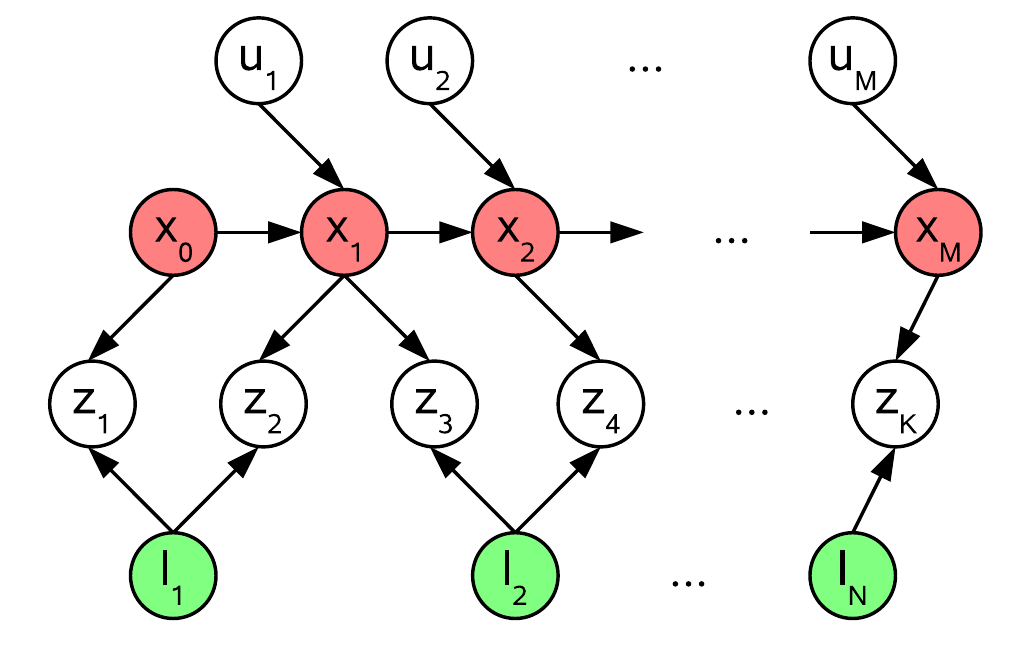
\includegraphics[width=0.45\textwidth]{images/kaess_slam_graph.png}
	\caption{
        SLAM graph with $x_i$ as the robot position at time step $i$. $l_j$ is the $j^{th}$ landmark. 
        $z_k$ is the $k^{th}$ by the robot measured landmark. $u_i$ is the control input at time step 
        $i$ which is for example odometry data \cite{kaess_isam:_2008}. For understanding: 
        At time step $1$ the robot position was $x_1$ and it measured landmark $l_1$ and $l_2$ 
        which can be seen by the measurements $z_2$ and $z_3$. The input from the control unit was $u_1$.
        }
	\label{fig:kaess_slam_graph}
\end{figure}